\documentclass[border=10pt]{standalone}

\usepackage{tikz}
\usepackage{tikzsymbols}
\usetikzlibrary{calc,patterns,shapes.geometric}

\def\centerarc[#1](#2)(#3:#4:#5){\draw[#1] ($(#2)+({#5*cos(#3)},{#5*sin(#3)})$) arc (#3:#4:#5);}

\begin{document}
	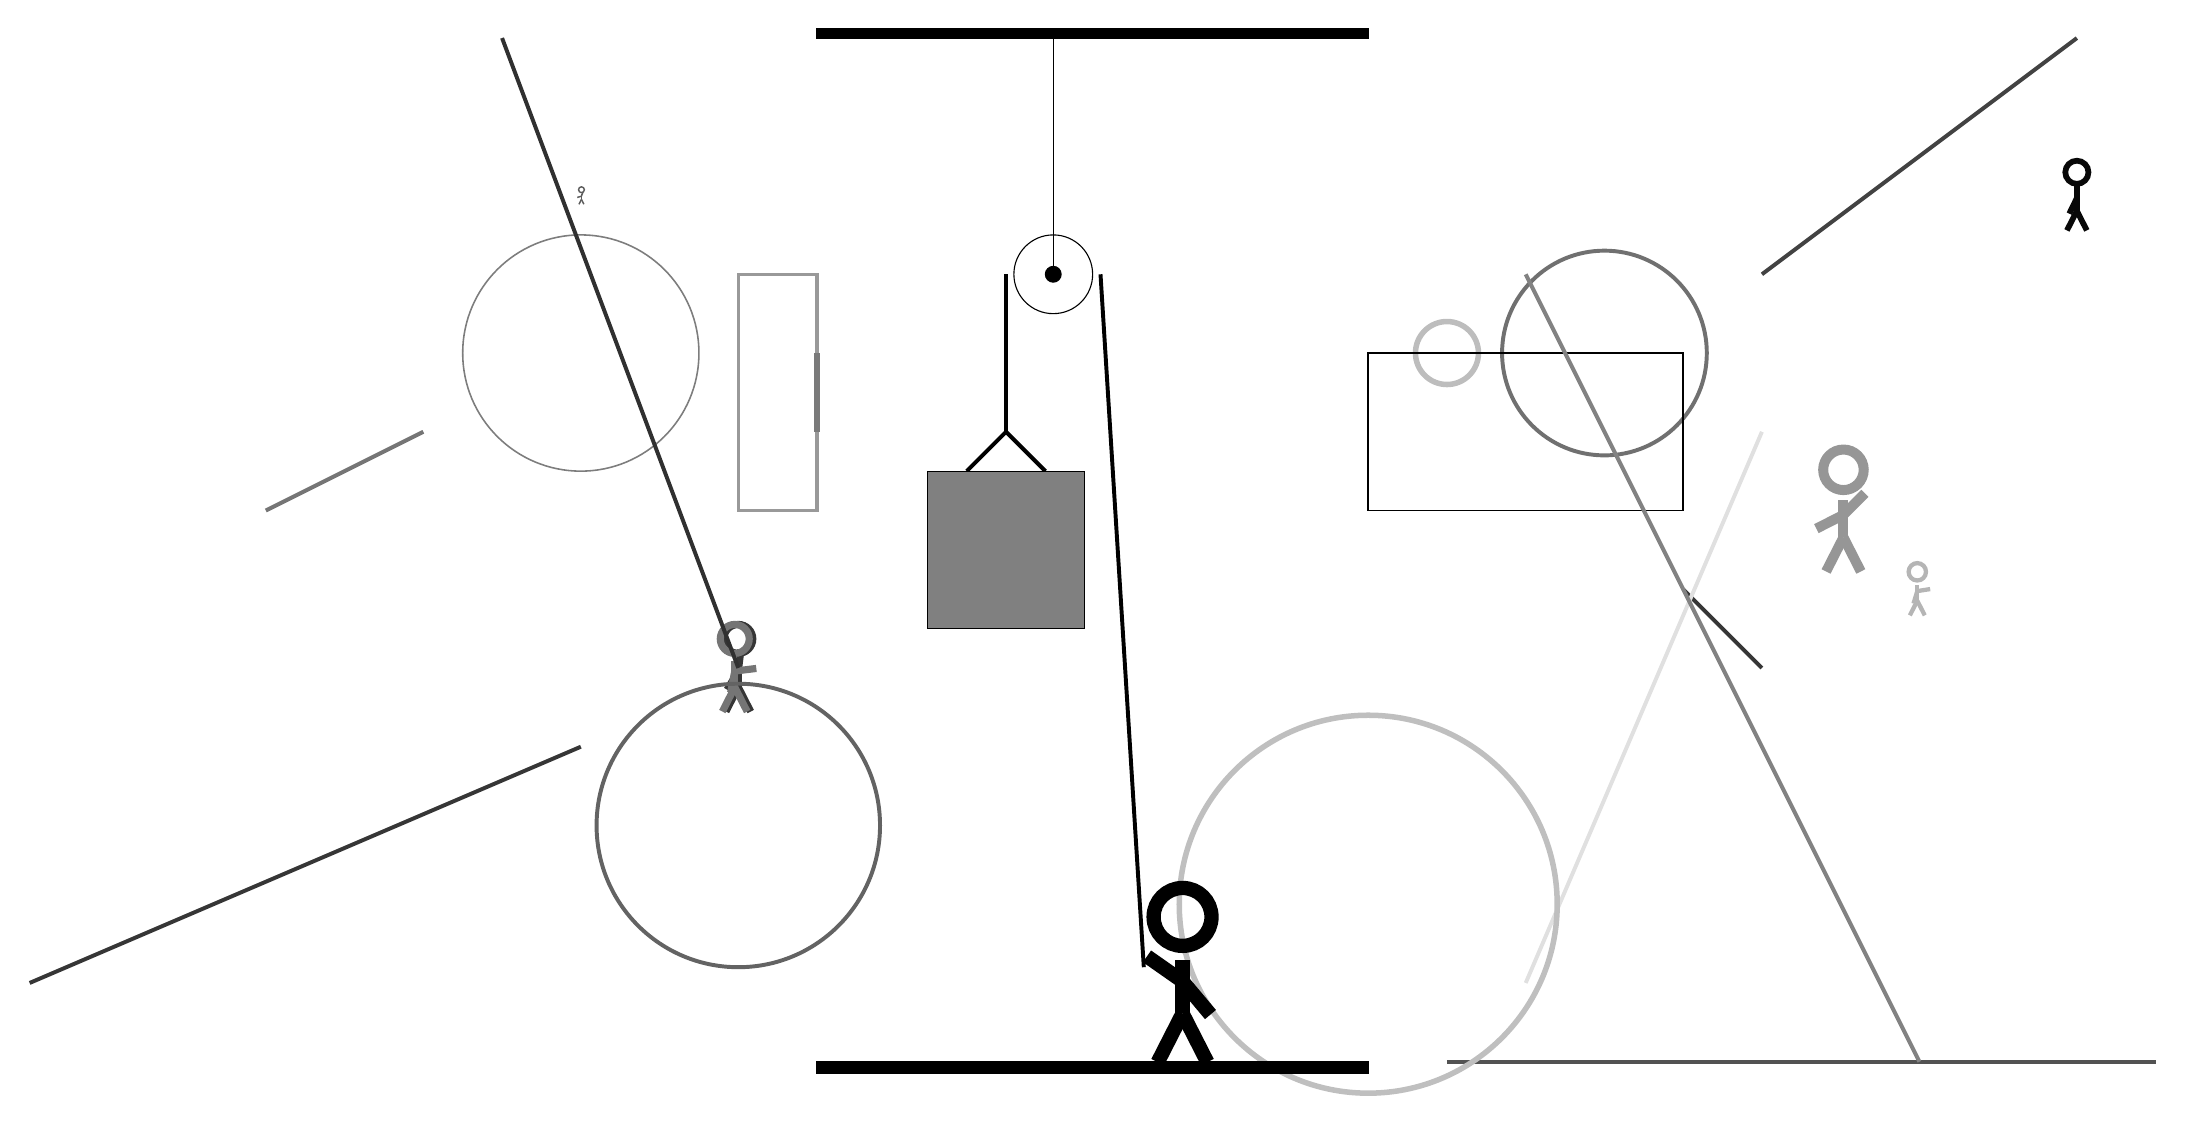
\begin{tikzpicture}
		%%%%% START %%%%%
		
		\draw[fill=black] (-2, 10) rectangle (5, 10.125);
		
		\draw [line width=0.2mm, color=black!51](-5, 6) circle (1.5);
		
		\draw[line width=0.4mm, color=black!40] (-2, 7) rectangle (-3, 4);
		\draw[line width=0.5mm, color=black!79](10, 2) -- (9, 3);
		\draw [line width=0.5mm, color=black!56](8, 6) circle (1.3);
		\draw [line width=0.7mm, color=black!26](6, 6) circle (0.4);
		
		\node[line width=0.6mm, color=black!79] at (-3, 2) {\Strichmaxerl[5][59][83]};
		\node[line width=0.7mm, color=black!29] at (12, 3) {\Strichmaxerl[3][73][9]};
		\draw[line width=0.5mm, color=black!12](10, 5) -- (7, -2);
		\node[line width=0.7mm, color=black!97] at (14, 8) {\Strichmaxerl[4][64][90]};
		
		\node[line width=0.4mm, color=black!41] at (11, 4) {\Strichmaxerl[7][27][45]};
		\draw[line width=0.2mm, color=black!100] (5, 6) rectangle (9, 4);
		\draw[line width=0.5mm, color=black!68](6, -3) -- (15, -3);
		\node[line width=0.7mm, color=black!54] at (-3, 2) {\Strichmaxerl[5][79][7]};
		\draw[line width=0.5mm, color=black!79](-5, 1) -- (-12, -2);
		\draw [line width=0.7mm, color=black!25](5, -1) circle (2.4);
		\node[line width=0.6mm, color=black!64] at (-5, 8) {\Strichmaxerl[1][17][70]};
		\draw[line width=0.7mm, color=black!52] (-2, 6) rectangle (-2, 5);
		
		\draw [line width=0.5mm, color=black!61](-3, 0) circle (1.8);
		\draw[line width=0.5mm, color=black!74](10, 7) -- (14, 10);
		
		\draw[line width=0.5mm, color=black!81](-3, 2) -- (-6, 10);
		\draw[line width=0.5mm, color=black!54](-7, 5) -- (-9, 4);
		
		\draw[line width=0.5mm, color=black!49](7, 7) -- (12, -3);
		
		\draw (1, 7) circle (0.5);
		\draw[fill=black] (1, 7) circle (0.1);
		\draw (1, 10) -- (1, 7);
		
		\draw[line width=0.5mm] (-0.1, 4.5) -- (0.4, 5.0) -- (0.9, 4.5);
		\draw[fill=black!50] (-0.6, 4.5) rectangle (1.4, 2.5);
		
		\draw[line width=0.5mm] (0.4, 7) -- (0.4, 5.0);
		\centerarc[line width=0.5mm](1, 7)(0:180:0.6);
		\draw[line width=0.5mm](1.6, 7) -- (2.15, -1.8);
		
		\node at (2.6, -1.9) {\Strichmaxerl[10][-35][-50]};
		
		\draw[fill=black] (-2, -3) rectangle (5, -3.15);
		
		%%%%% END %%%%%
	\end{tikzpicture}
\end{document}